
%(BEGIN_QUESTION)
% Copyright 2008, Tony R. Kuphaldt, released under the Creative Commons Attribution License (v 1.0)
% This means you may do almost anything with this work of mine, so long as you give me proper credit

What will happen to the voltage drops across each resistor in this circuit if resistor R1 fails open?

$$\includegraphics[width=15.5cm]{i03152x01.eps}$$

\begin{itemize}
\item{} $V_{R1}$ = ({\it increase}, {\it decrease}, or {\it stay the same})
\vskip 10pt
\item{} $V_{R2}$ = ({\it increase}, {\it decrease}, or {\it stay the same})
\vskip 10pt
\item{} $V_{R3}$ = ({\it increase}, {\it decrease}, or {\it stay the same})
\vskip 10pt
\item{} $V_{R4}$ = ({\it increase}, {\it decrease}, or {\it stay the same})
\end{itemize}

\vskip 20pt

Be sure to explain your reasoning for the answers you give!

\vfil 

\underbar{file i03152}
\eject
%(END_QUESTION)





%(BEGIN_ANSWER)

This is a graded question -- no answers or hints given!

%(END_ANSWER)





%(BEGIN_NOTES)

\begin{itemize}
\item{} $V_{R1}$ will {\bf increase} to full supply voltage
\vskip 10pt
\item{} $V_{R2}$ will {\bf decrease} to zero
\vskip 10pt
\item{} $V_{R3}$ will {\bf decrease} to zero
\vskip 10pt
\item{} $V_{R4}$ will {\bf decrease} to zero
\end{itemize}

If R1 fails open, current will be interrupted to all other resistors in the network.  This will result in those resistors' voltage drops becoming zero, while full supply voltage gets dropped across (open) R1.

%INDEX% Pictorial circuit review (series-parallel resistor network)

%(END_NOTES)


